%4章提案
\begin{comment}
\section{既存手法の問題点}
既存の監視手法として次のような手法がある.
\begin{itemize}
\item 監視サーバからの問い合わせによる監視\\
	Ping,SNMPによる問い合わせ等がこの手法にあたる.
\item 機器からの通知に基づく監視\\
	SNMPTrapによる通知がこの手法である.
\end{itemize}
\medskip

監視サーバからの問い合わせによる監視をIoTサービスに適応した場合,次のような問題がある.
\begin{itemize}
\item IoT機器が接続するネットワークが,プライベートアドレスを使用している場合がある\\
	IoT機器が接続するネットワークがプライベートアドレスである場合,監視サーバから問い合わせを行うことができず,監視することができない.
\item IoT機器が接続するネットワークにセキュリティの設定が施されている場合がある\\
	特に,インターネットからの特定ポートに対するアクセスをブロックしている場合がある.
	この場合も,監視サーバからの問い合わせを行うことが出来ないため,監視することが出来ない.
\item IoT機器が移動する場合がある\\
	IoT機器は移動する物に取り付けられる場合がある.
	この場合,IoT機器が接続するネットワークが頻繁にかわるため,監視サーバが問い合わせを行う宛先を頻繁に更新しなければならない.
	また,複数の機器が移動を繰り返す中で,監視サーバとのやり取りに混乱が生じる.
\end{itemize}
このため,監視サーバからの問い合わせによる監視は用いることができない.
\medskip

一方,機器からの通知では,これら機器が接続されるネットワークに起因する問題を解決できる.
しかし,各IoT機器に対し個別のIDを設定する必要が有り,IoT機器が大量であることから大きな負担となる.
また,どちらの手法を取るにしても,機器監視サーバへの登録作業は行う必要が有り,負担となる.
\end{comment}


\section{IoT機器監視・管理サービスの提案}
IoTサービスの円滑な提供の為には,IoTサービスの構造を維持する必要が有り,そのために,IoT機器を監視する必要がある.
IoT機が接続するネットワークが,プライベートアドレスを利用している等,多様であることから,機器からの通知による監視手法を取る必要がある.
しかし,IoTサービスにおいて,IoT機器は多量に使用されることや,頻繁な交換・追加がありうることから,
IoT機器へ個別の設定をすること,監視サーバへIoT機器を登録することが大きな負担となっている.
\medskip

\begin{figure}[htbp]
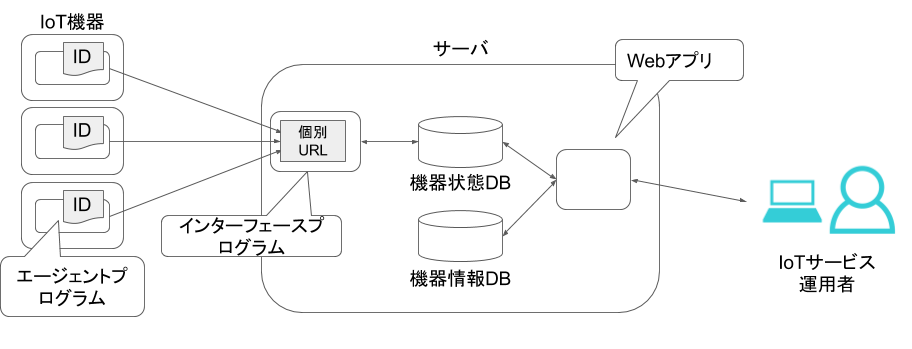
\includegraphics[width=16cm]{images/prop_diag.png}
\caption{サービス構成図}
\label{fig:prop_diag}
\end{figure}
そこで私は,これら負担はIoT機器と監視サーバに設定が分散していることが原因と考え,設定を監視サーバにて一元的に管理し,IoT機器への設定の省力化を提案し,サービスを開発する.
このサービスの利用者は,提案するサービスから,機器追加用のトークンを受け取り,各IoT機器に対して同一のトークンを設定し,提供するプログラムを作動させる.
提供するプログラムは,監視サーバに対して,このトークンを送信し,返答として個別のIDを受け取り,自身に設定する.
サーバでは,トークンの有効性を検証し,機器の追加を自動的に行う.
図\ref{fig:prop_diag}は,提案するサービスの構成図である.
\newpage

\begin{figure}[htbp]
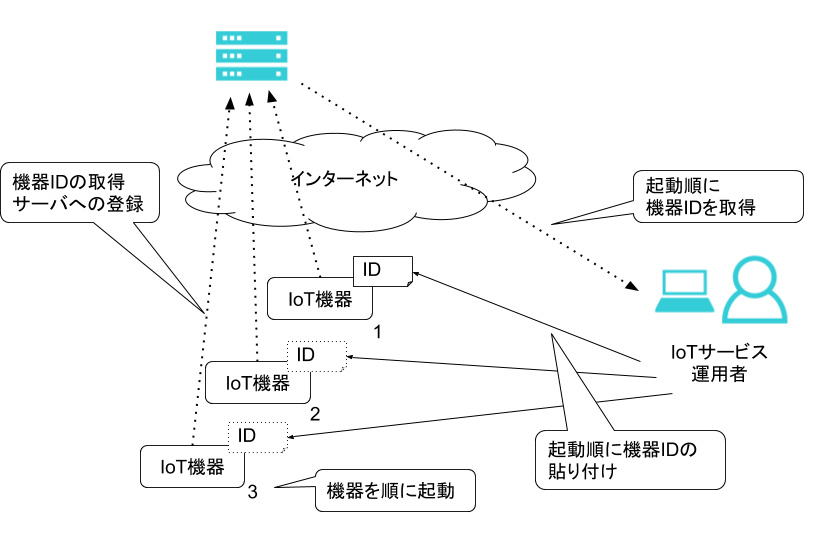
\includegraphics[width=16cm]{images/prop_diag2.png}
\caption{サービス構成図}
\label{fig:prop_diag2}
\end{figure}
図\ref{fig:prop_diag2}の様にプログラムを作動させた順に,機器の監視サービスへの登録を確認し,機器に対してIDの貼り付け等を行う.
また,IoT機器上で動作する提供プログラムは,定期的に監視サーバに対しネットワークの状態や稼働状況等を報告することで,監視を行う.

これにより,監視サーバへ各IoT機器を登録する負担と,IoT機器へ個別の設定を行うことを省力化する.
さらに,通知型でhttpsを用いた通信により,ネットワークの多様性に対応する.
また,サービスとして提供することで,従来では不可欠であった監視サーバの構築作業の負担も解決することができる.

\begin{comment}

IoT機器からの通知に基づいた,設定不要の独立した状態監視のためのサービスを提案する.
機器から通知を送ることで,IoT機器の接続されるネットワークが,プライベートアドレスを使用していても監視可能であること,ネットワークが違っていても一つの画面で確認できることを満たす.
また,状態監視の為のサービスを独立させることで,IoTサービスの変更が不要であることや,監視サーバを立てる必要が無いことを満たす.
IoT機器への設定の必要性については,あらかじめ,IoT機器自体に存在する識別IDを用いることとする.
こうすることで,監視サーバに対して,設定をする必要がなくなる.



このように,今後使用するIoT機器が増えていくことを考えると,現状の手動での監視は負担となる.
そこで,新規にIoT機器の監視に汎用的に使用できるシステムを開発し,サービスとして提供することで,問題の解決が図れるのではないかと考えた.
実験と聞き取りから得られた要件を以下にまとめる.
\begin{itemize}
\item 機器が起動し動作していることが確認できること
\item CPUの温度等も確認できると良い
\item 各機器に対する監視に関わる設定の簡略化もできたら良い
\item 機器の異常をメールなどで知らせることができたら良い
\item 機器の状態をIoTサービスごとに管理したい
\end{itemize}
\end{comment}

